% !TEX root = ../../thesis.tex

\cleartoleftpage
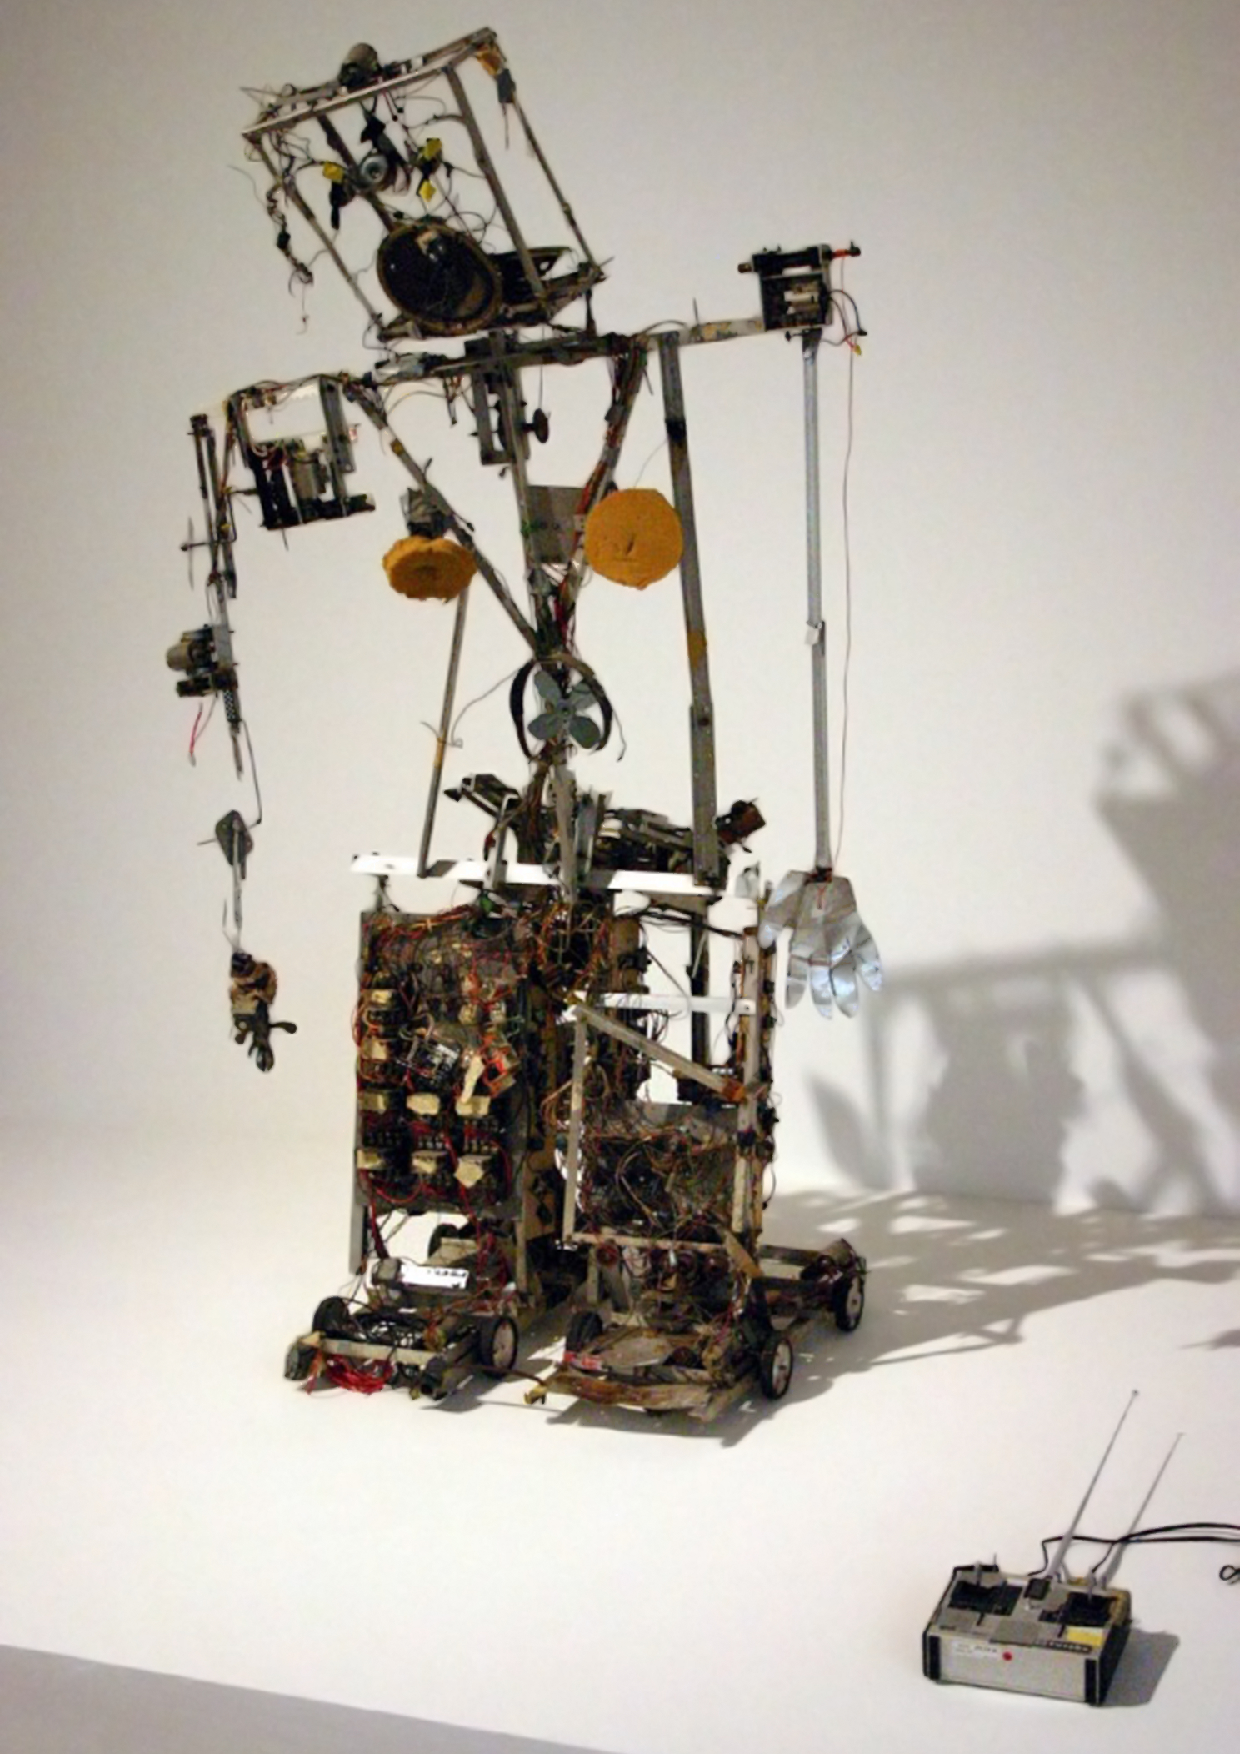
\includepdf{../media/chapter_illustration/Nam_Jun_Paik}

\chapter{Art} % (fold)
\label{cha:art}

\cleanchapterquote{Artists and mathematicians have a lot of points in common in their way of working in the end,. There is this important role for the mathematician and for scientists generally, of inspiration, culture, exchange of ideas, schools of thought which change over time or which vary from one country to another, and at the same time, scientific universality is the same as that found in the arts.}{Cédric Villani}



\section{Introduction} % (fold)

Science and Art have been intermingled for ages. Leonard da Vinci\footnote{Humanist artist who lived during the Renaissance, Leonardo da Vinci had many different hats. He was a painter, sculptor and musician but also an engineer, mathematician, physicist, biologist, astrologer, architect and urban planner. Famous today for his painting, he also left behind visionary flying and war machines.} is a meaningful example of the very existence of such a scientist-artist status. Contrary to popular opinion, the two worlds are more in agreement with each other than they are in opposition. Indeed, in both areas, although the methods of investigation and processes implemented to experiment the world may differ, both artists and scientists are motivated toward the same goal: understanding the world around them to share and exchange knowledge with others.


Several results and technologies coming from scientific applications have been transformed into material resources, instrumental, or technical processes for Art. For example, chronophotography, invented by Etienne Jules Marey and Eadweard Muybridge to study human and animal locomotion (see \figurename~\ref{fig:marey_chronophotography}), has been a source of inspiration for Futurists\footnote{At the time of the Futurists, Art sought to express the dynamism of modern life and the representation of contemporary society: they consider movement and speed as the most significant emerging phenomena of the twentieth century.} who reproduce in their work the decomposition of movement visible in chronophotographies (see \figurename~\ref{fig:duchamp_chronophotography} and \figurename~\ref{fig:russolo_chronophotography}). Futurists are proponents of the fusion of art with technology and the natural sciences: \emph{"The method of constructing a machine is similar to the method of undertaking a work of art"}~\parencite{severini1917machinisme}.


\begin{figure}[!tb]
\centering
    \subfloat[][]{\label{fig:marey_chronophotography}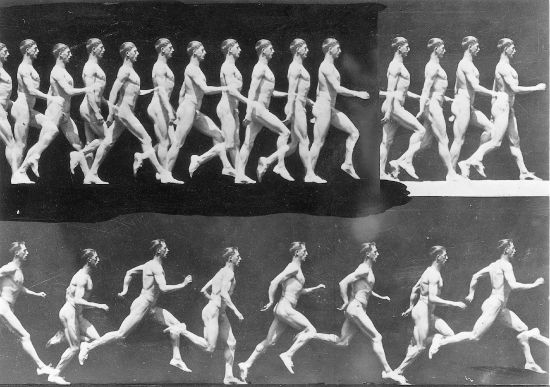
\includegraphics[width=0.8\linewidth]{chronophotography.jpg}}\\
    \subfloat[][Marcel Duchamp, \emph{Nu descendant un escalier}, oil on canvas, 146 x 89 cm (1912) - Philadelphia Museum of Art, Philadelphie (États-Unis).]{\label{fig:duchamp_chronophotography}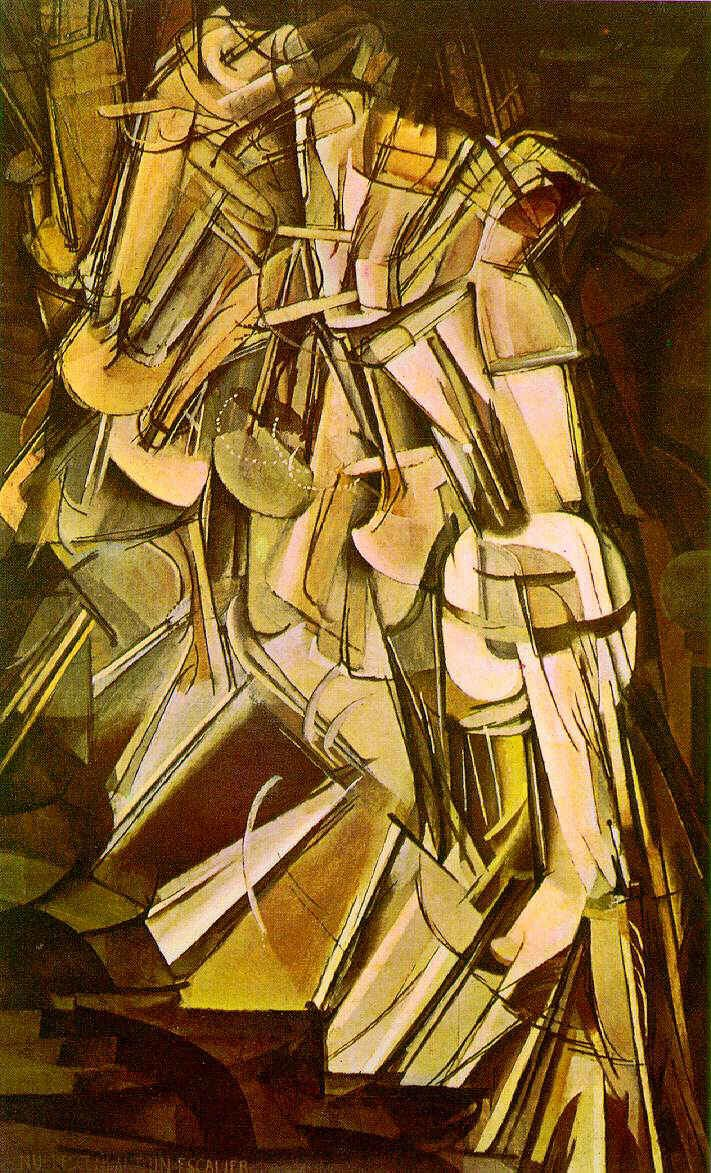
\includegraphics[height=6cm]{chronophotography_duchamp.jpg}}
    \hfil
    \subfloat[][Luigi Russolo, \emph{Dynamisme d’une automobile}, 1912 – Centre Georges Pompidou.]{\label{fig:russolo_chronophotography}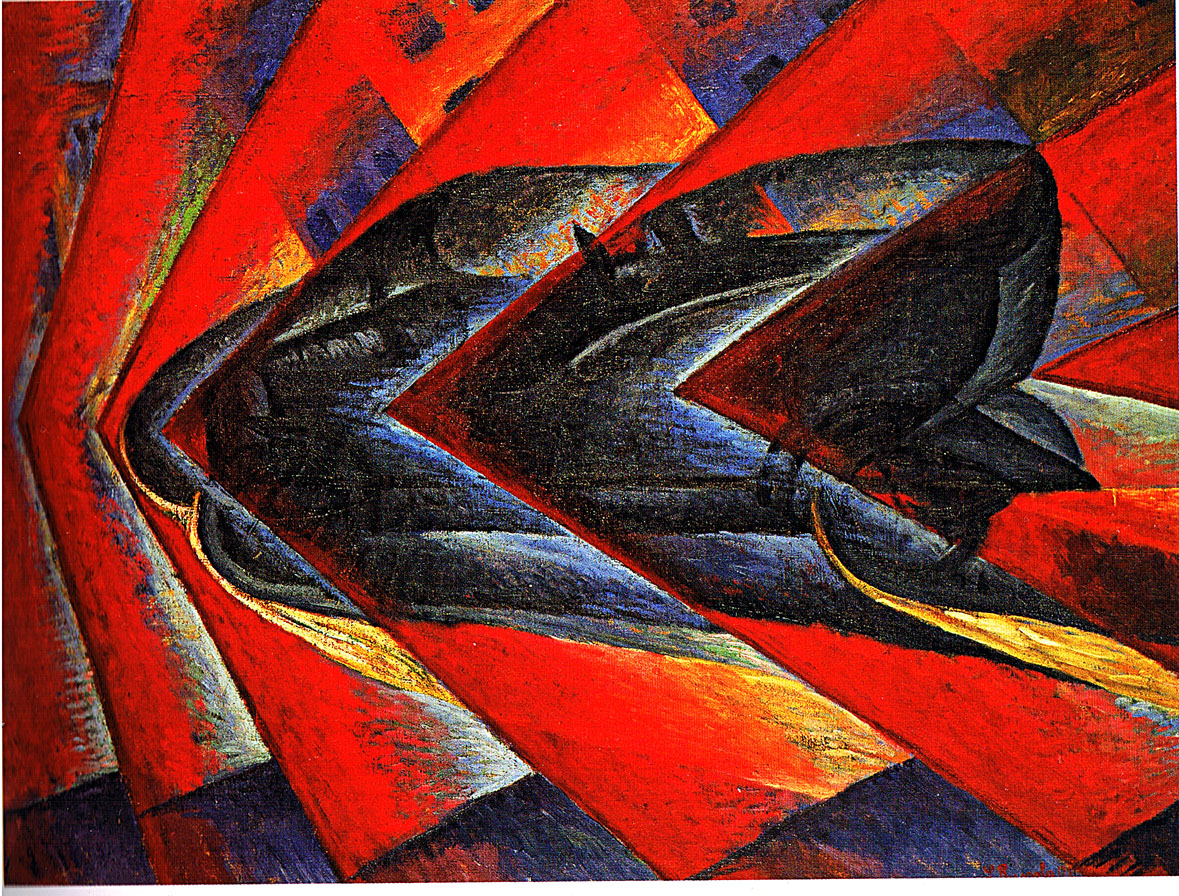
\includegraphics[height=6cm]{chronophotography_russolo.jpg}}
    \caption{}
    \label{fig:chronophotography_history}
\end{figure}


If Science proves to be a source of inspiration for Art, in return, Art is also involved in Science and plays a major role in providing the general public with an understandable representation of complex scientific discoveries or concepts. Indeed when mixed with science and technical applications, artistic creation also serves as an original vector of mediation to reach the uninitiated. The sensory experience brought by a work of art favors the appropriation of innovative technology or research results, especially because it demystifies the complexity of the mechanisms involved with the sensory approach and concrete production is more easily comprehensible than theoretical explanations. In doing so, Art often helps to understand issues or potential uses, defuse fears of novelty and expand distribution.
Astrophysics is a great example of this. None of us will ever see a giant black hole or the sun becoming a red giant. In this context, artistic contributions are vital as it would be difficult to arouse the attention and interest needed for funding of such expansive research without appropriate mediation.


In this direction, the Flowers team in collaboration with the artist and movie-maker David Lynch lead a project called "ergo robots" (see \figurename~\ref{fig:ergo_robot}) as part of the "Mathematics: A Beautiful Elsewhere"\footnote{Mathematics: A Beautiful Elsewhere is a unique exhibition created by the Fondation Cartier pour l’art contemporain with the aim of offering visitors, to use the mathematician Alexandre Grothendieck’s expression, “a sudden change of scenery.” The Fondation Cartier opened its doors to the mathematics community and invited a number of artists to accompany them. They are the artisans and thinkers, the explorers and builders of this exhibition. More info on \url{http://fondation.cartier.com/en/art-contemporain/26/exhibitions/294/all-the-exhibitions/89/mathematics-a-beautiful-elsewhere/}} exhibition in 2011 at the Cartier Foundation for Contemporary Art. The experiment of the Flowers team addressed artificial curiosity, the embodiment and discovery of language in robots and was aimed at, among other goals, interaction with a non-science-enthusiast audience. In this experiment the collaboration between science and art has revealed art as a medium and tool for scientific mediation.

\begin{figure}[!tb]
\centering
    \subfloat[][]{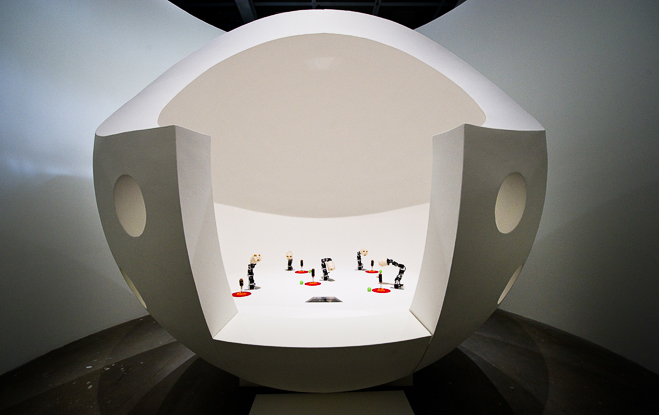
\includegraphics[height=4.2cm]{ErgoRobotFondationCartier.jpg}}
    \hfil
    \subfloat[][]{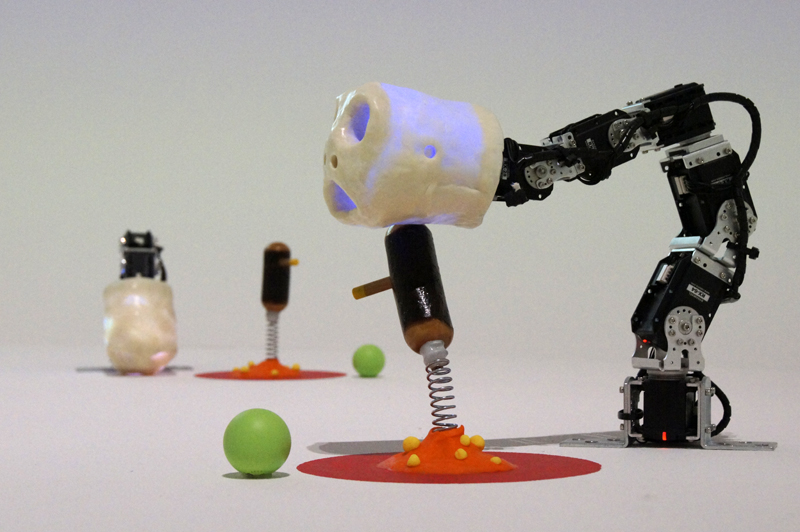
\includegraphics[height=4.2cm]{ErgoRobots13.jpg}}
    \caption{}
    \label{fig:ergo_robot}
\end{figure}


Yet this kind of collaboration between a scientific laboratory and artists is rare.
We indeed notice the recent increase in complexity and in the level of culture/education needed to understand the latest work coming out of these two worlds\footnote{C. P. Snow explained in "two culture" theory (REF) that people in humanities and art, and those in science had developed sufficiently different languages and world views that they did not understand each other.}. Without knowledge of art history, it is sometimes difficult for a scientist to understand contemporary works of art. Likewise, it is somewhat difficult for artists\footnote{It should be noted that the arts community hosts diverse profiles of artists. Curiously (in many cases), works combining art and science are creations of artists who are none other than converted scientists.} to appreciate the scientific work because of the technical complexity involved.
Interaction is indeed sometimes difficult because we do not speak the same language, but robots raise countless issues and challenges and even if some of them are very technical and require the use of mathematical formalisms to be explored, a wide range of problems can be addressed with the relevant collaboration of artists.

What interests us particularly, and relates to this research, is the alternative perspectives artists bring to the dialogue on  the societal impact of robots or human-robot interaction, opening new research axes or new ways of exploring them.
One emblematic  loan  from art is robotic emotion. The expression of emotions in a virtual machine or humanoid is a dual representation: firstly, it depends on how the human emotional functions have been understood; secondly, it is based on a representation of the iconography of emotions. These two representations are well mastered by artists. Brilliant examples can be found in cinema (see \figurename~\ref{fig:robot_emotion_cinema}). Only using basic beep-based sounds, R2D2 is able to communicate and is actually more appealing than C3PO, a classic humanoid robot speaking hundreds of languages. Another impressive example is Wall-E, without an actual human face, the animators have been able to create a wide range of intense emotions.
These two examples show how roboticists could benefit from artists’ expertise in the field of sensitivity in order to design more expressive robots.


\begin{figure}[tb]
\centering
    \subfloat[][The C3-PO and R2D2 robots in Star Wars: A new hope]{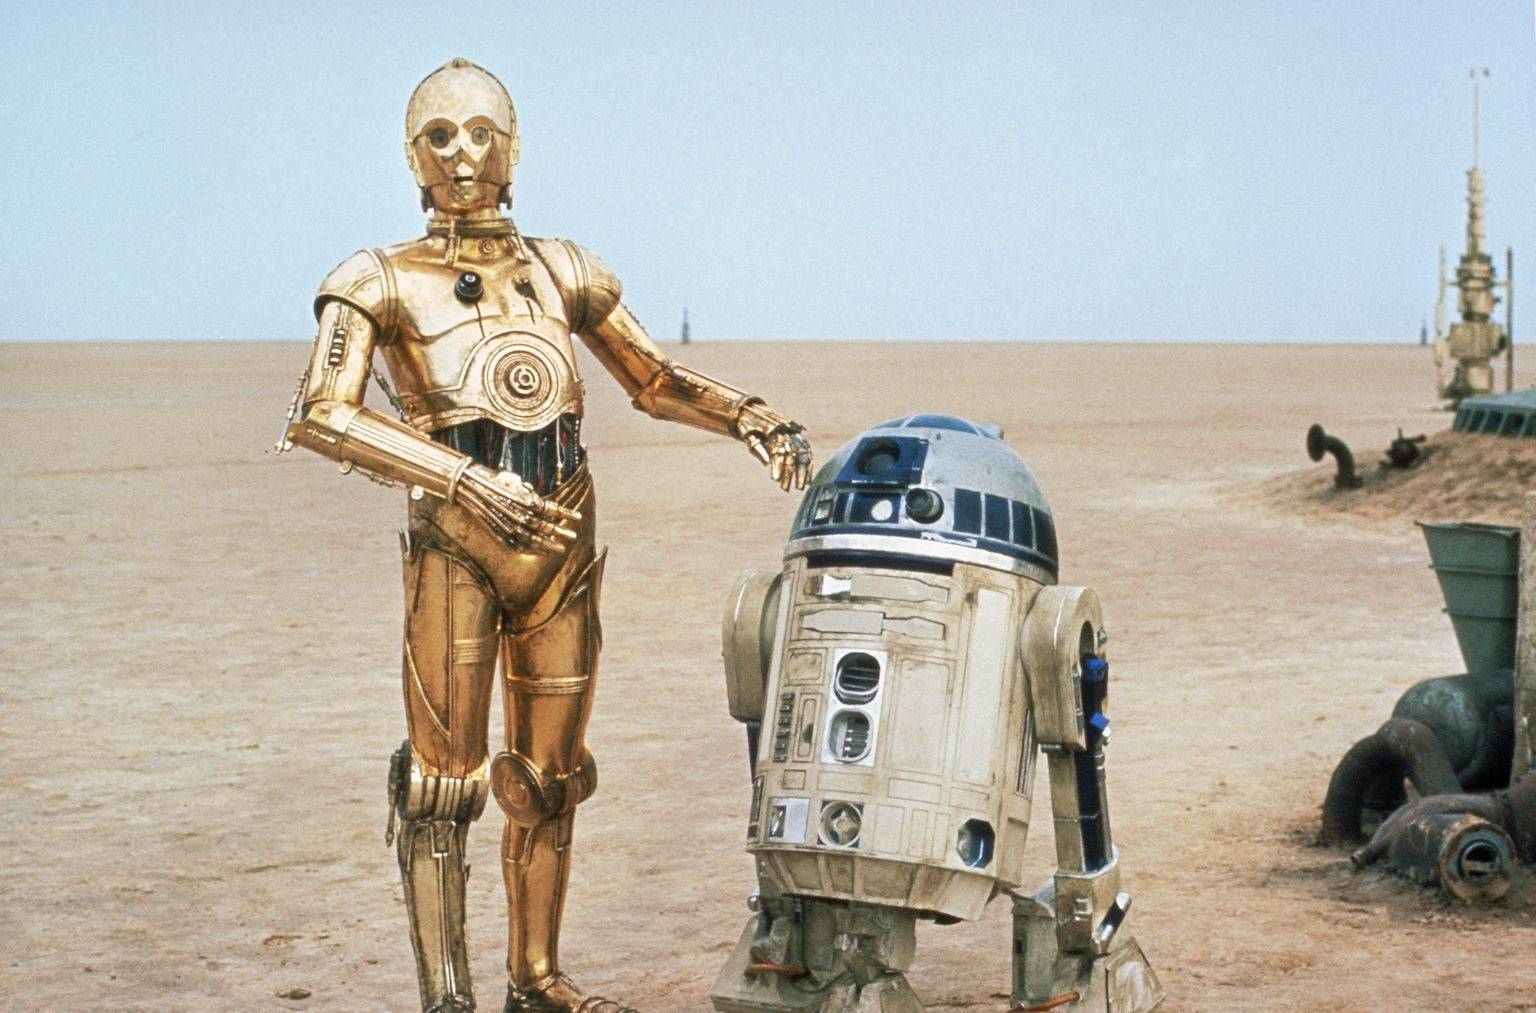
\includegraphics[height=4.5cm]{r2d2.jpg}}
    \hfil
    \subfloat[][Wall-E being curious about a Rubik's cube]{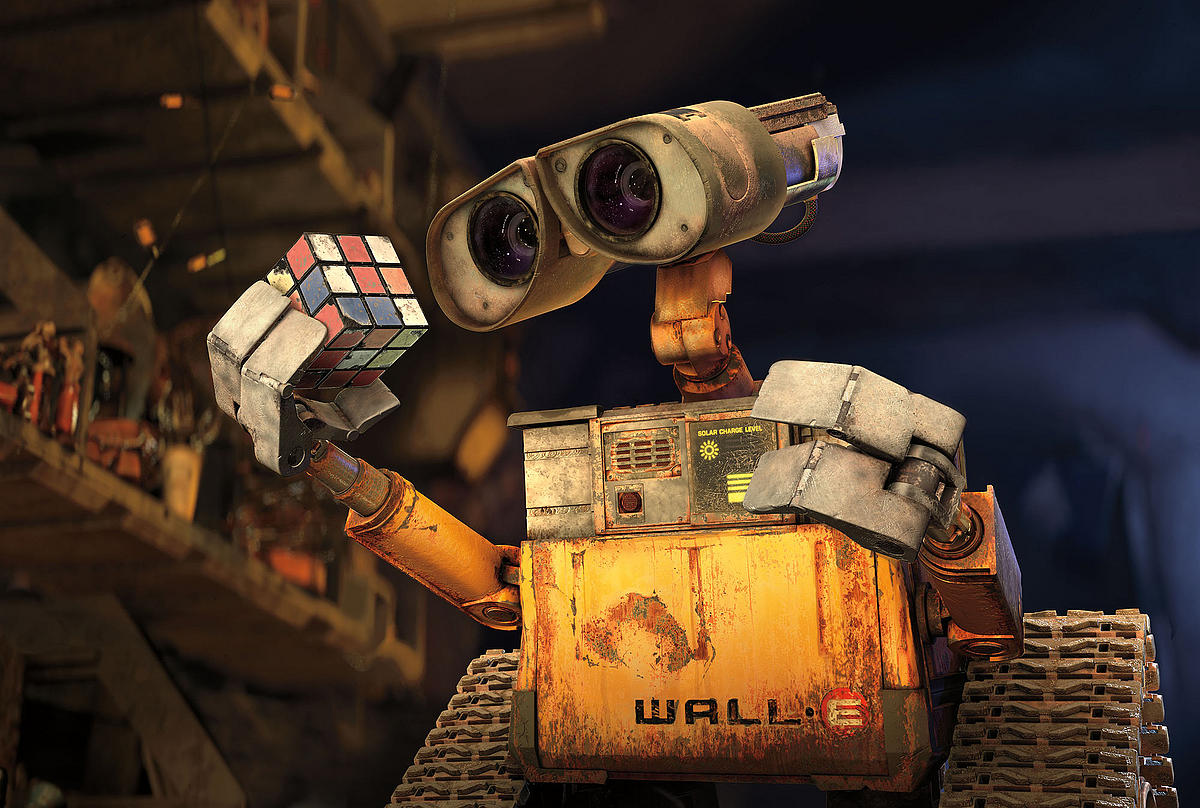
\includegraphics[height=4.5cm]{Wall-E.jpg}}
    \caption{}
    \label{fig:robot_emotion_cinema}
\end{figure}


\section{Motivation } % (fold)
\label{sec:motivation}

Poppy is fully hackable, so artists could be interested by the freedom for exploration they have to change the morphology or the design of the robot, add new features or sensors, change its behaviour and so on. Also, Poppy is designed to be experimental-proof (see section REF), it is quite robust and easily reparable so it can be used in rather difficult conditions.

As we discussed previously, the artistic community is a rich source of inspiration and can provide new perspectives on scientific and technological questions. The work of artists is complementary to that of scientists. In the open source robotic community we are trying to set up, this complementarity is a great opportunity that we want to encourage by making the robot accessible for non-robotic-expert users.

While it is a real desire to make Poppy accessible and useful for the artistic community, we needed to gain experience of such uses in an actual artistic project to evaluate how relevant Poppy is for artists and what artists can bring into the development of the Poppy project.


\section{The \emph{Êtres et numérique} project} % (fold)

The first artistic project in which Poppy is involved is entitled "Êtres et Numérique". This contemporary art project focuses on ways of representing and interacting with movement digitally. It is led by the artists\footnote{Comacina Capsule Creative, \url{http://www.comacina.org/}} Amandine Braconnier (mixed media artist) and Marie-Aline Villard (dancer-researcher), and supervised by Thomas Desmaison (Point barre\footnote{\url{http://www.pointbarre.biz/}}) from the Fabrik Pola\footnote{\url{http://www.pola.fr/}}.

\begin{figure}[tb]
    \begin{center}
        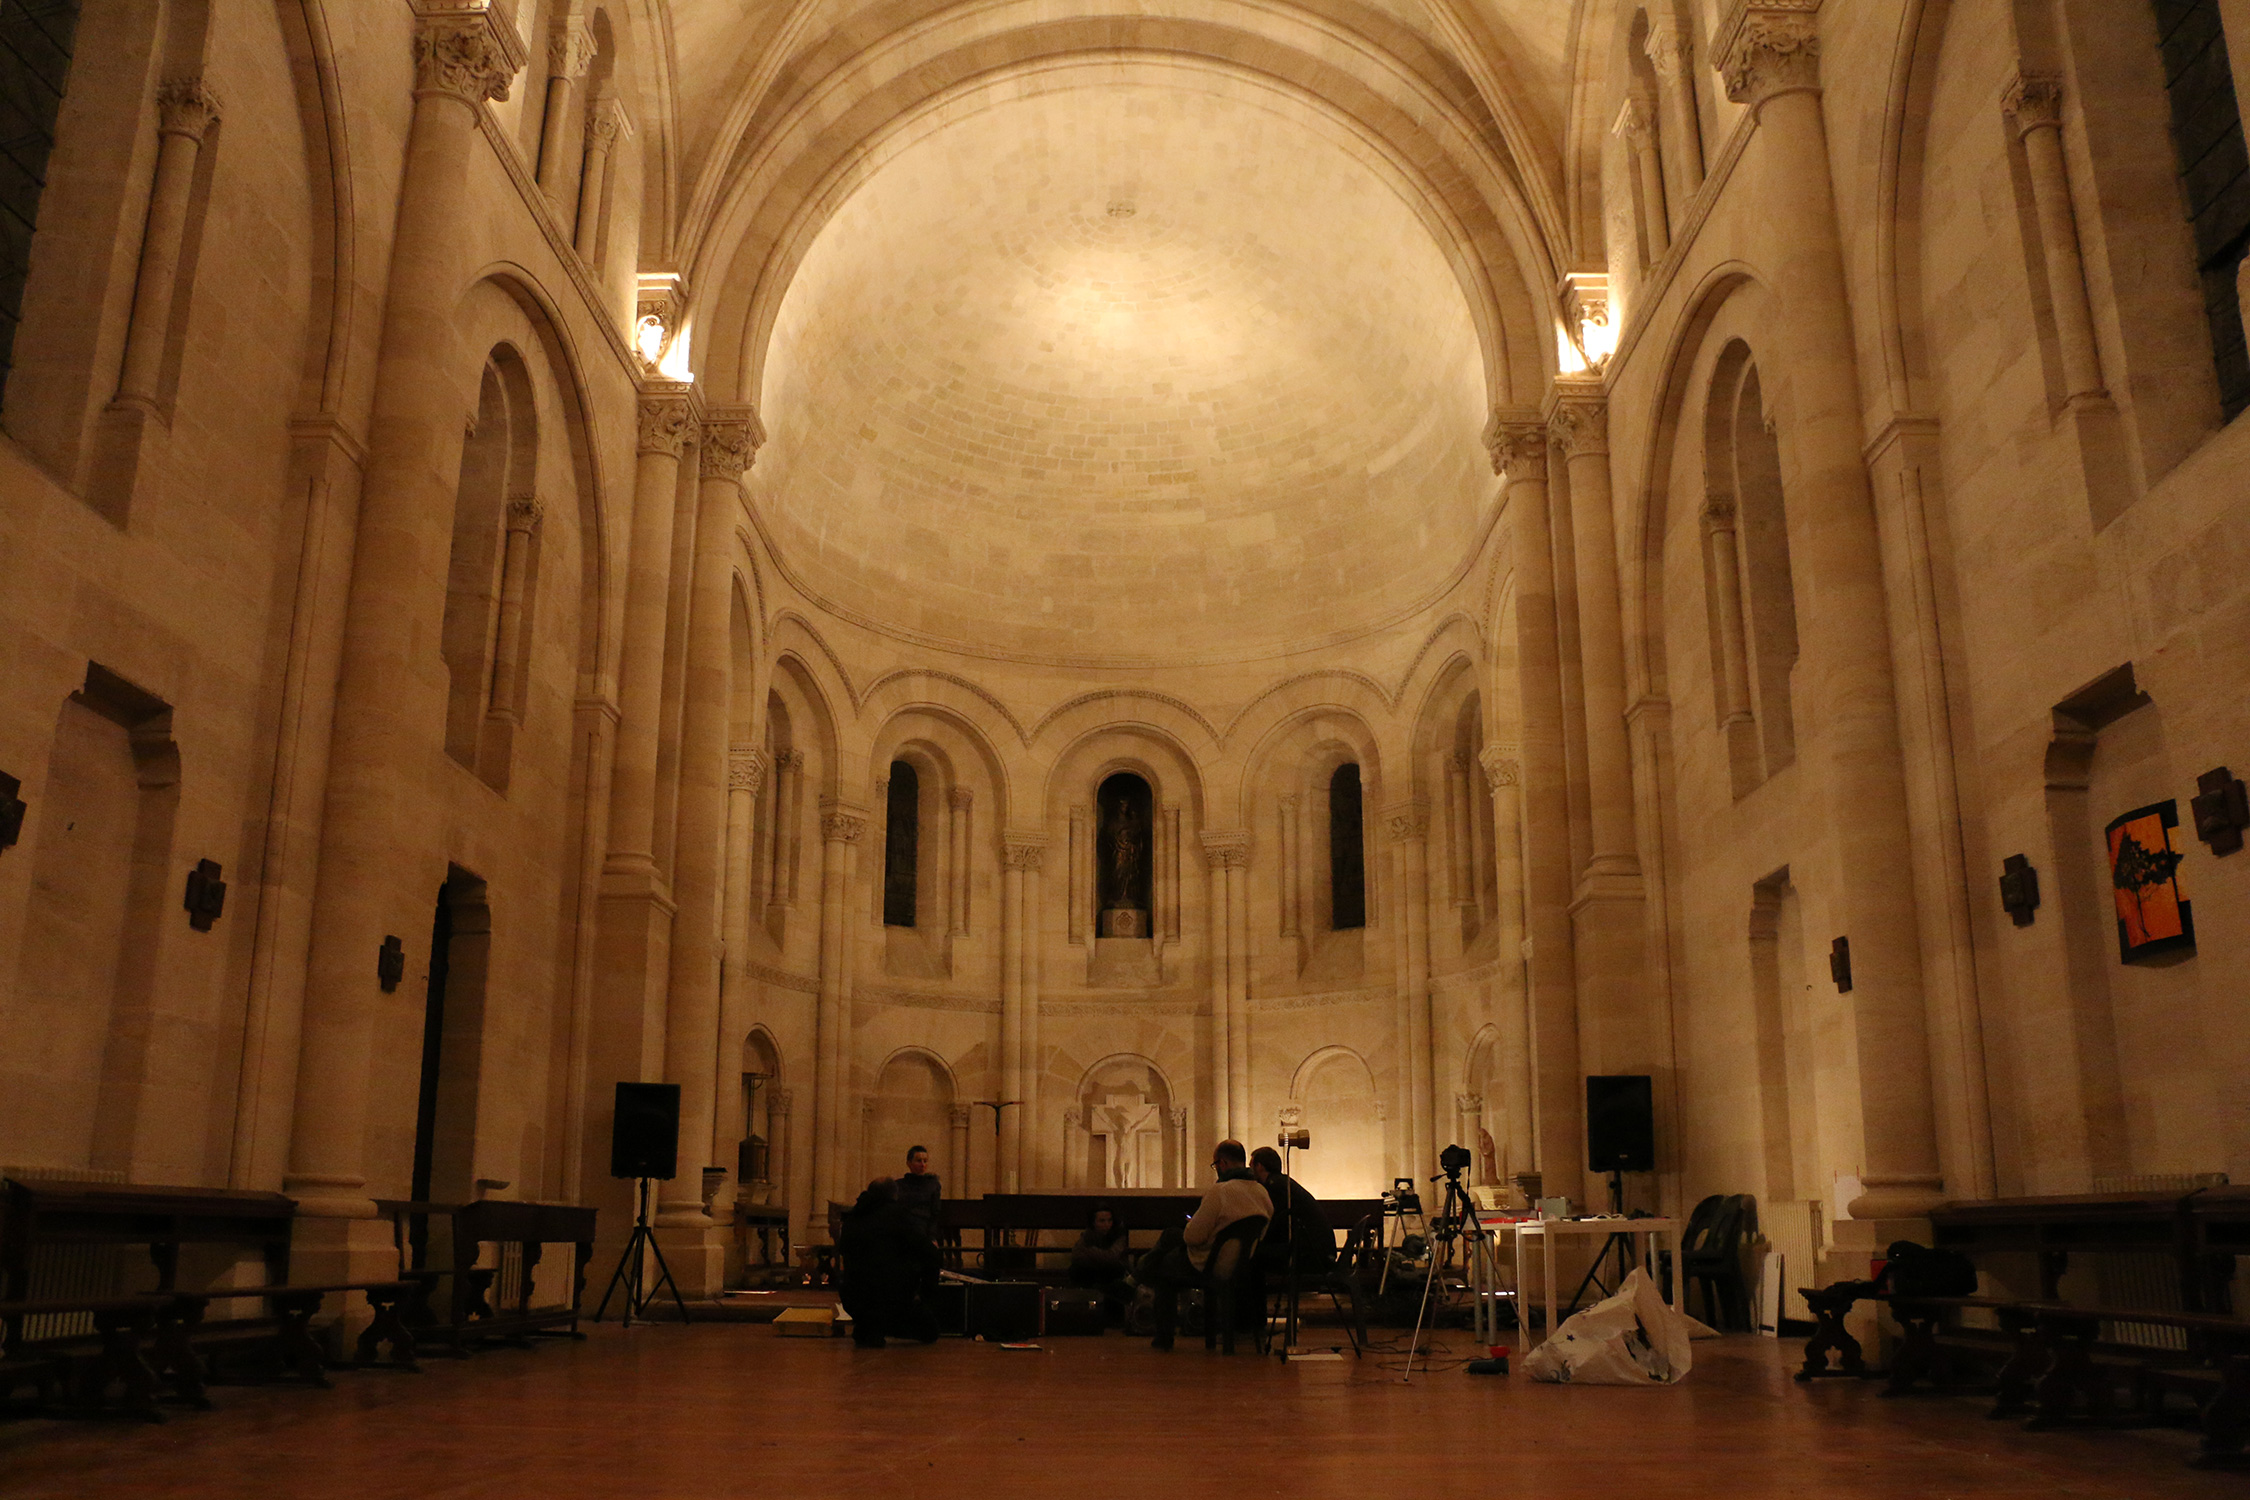
\includegraphics[width=0.8\linewidth]{saintonge_chapel.jpg}
    \end{center}
    \caption{The "Êtres et numérique" residency and performances took place in the gorgeous chapel of the \emph{lycée des metiers Sainte Famille Saintonge}}
    \label{fig:saintonge_chapel}
\end{figure}

\textbf{A video trailer is available here: \url{https://vimeo.com/92281019}.}

For these artists, the use of a hackable humanoid robot is a whole expressive tool that opens up new horizons. Indeed, a robot permits to dissect and analyse movements. It allows them to play around with its body and model gestures as one could sculpt shapes in clay. Also, the use of non-rigid actuation allows the emergence of unpredictable and unexpected movement, while Poppy under-actuation ensures safe physical interaction.


The first "Êtres et Numérique" work took the form of a ten-day art-science-mediation residency involving members of the Poppy project, the artists with the participation of Jean Marc Weber (music composer) and was supported by the Aquitaine Region. It took place in a Bordeaux (Fr) high school (Lycée Saintonge Sainte Famille\footnote{\url{http://www.lyceesaintefamille.com/}}), which made its gorgeous chapel available (see \figurename~\ref{fig:saintonge_chapel}) for the artistic performances.


This residency was really important for the poppy project: it was the first trial of a real artistic application of Poppy, bringing to light new potential applications and bugs.

The main objective of this first residency was the preparation of a dance performance using the passive properties of Poppy and a physical human-robot interaction with the dancer, but several experiments has been conducted aside from this common thread.


\subsection{Artistic exploration} % (fold)

The residency week was a playground of exploration for both Poppy and us. The artists were especially interested in how to represent movement and interaction between humans and robots.

A first experiment consisted in visually tracing over a canvas the combined movement of the dancer and the robot (see \figurename~\ref{fig:residency_canvas}). To do so, we dressed Poppy to protect it against dirt (see \figurename~\ref{fig:poppy_dressed}). Then M. A. Villard danced with Poppy on canvas covered with pigments (see \figurename~\ref{fig:poppy_playing_with_pigment}). These dancing movements were captured by pigment traces and created paintings of sorts (see \figurename~\ref{fig:pigment_traces}). The whole collection was exhibited in the chapel (see \figurename~\ref{fig:whole_canvas_collection}.

\begin{figure}[tb]
\centering
    \subfloat[][Poppy dressed to protect it against dirt]{\label{fig:poppy_dressed}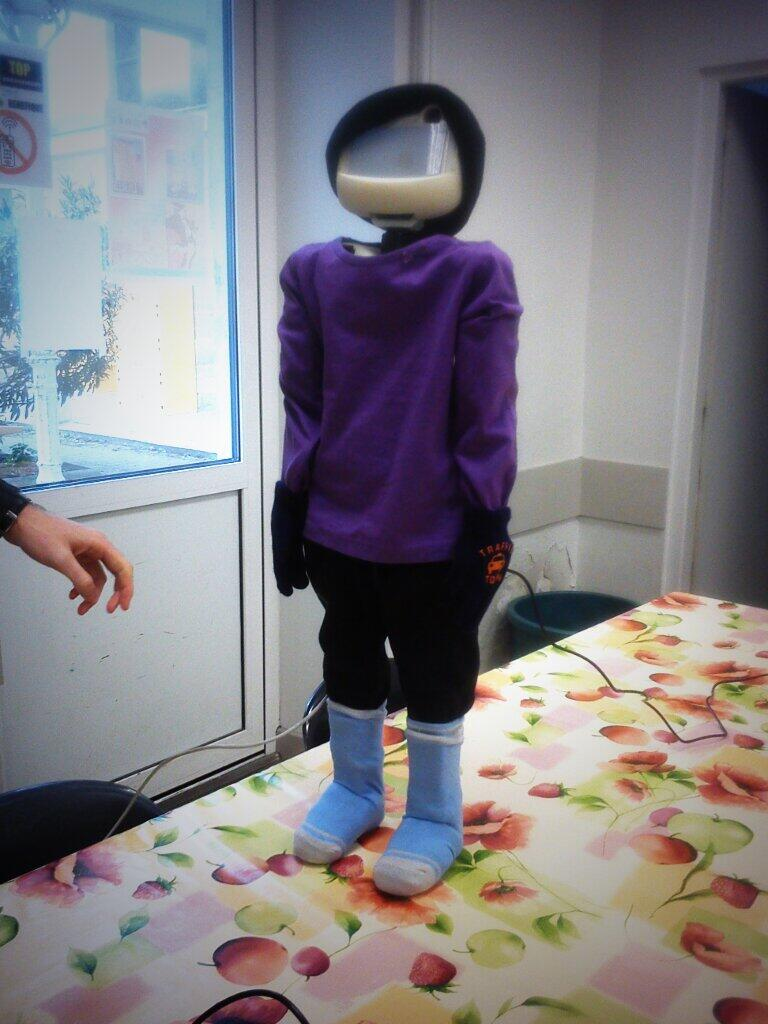
\includegraphics[height=6cm]{poppy_4ans.jpg}}
    \hfil
    \subfloat[][Poppy and the dancer playing on canvas covered with pigments]{\label{fig:poppy_playing_with_pigment}\includegraphics[height=6cm]{IMG_0191.jpg}}\\
    \subfloat[][Result of this human-robot interaction]{\label{fig:pigment_traces}\includegraphics[height=6cm]{_MG_7996.jpg}}
    \hfil
    \subfloat[][The whole canvas collection was exhibited in the chapel]{\label{fig:whole_canvas_collection}\includegraphics[height=6cm]{IMG_0518.jpg}}
    \caption{Movement }
    \label{fig:residency_canvas}
\end{figure}

An alternative way of representing movement is to transform motion into sounds. This is the playground of Jean Marc Weber, an electro-acoustician and music-composer, creating music using the interaction between probabilistic composer and body space motions. To do so, he created plugins allowing the use of webcam, Kinect or Leap motion with the music-software Usine\footnote{usine TODO}. For this purpose we explored both the use of Kinect and Leap motion with Poppy.

When Poppy is dressed it can be tracked by Kinect sensors\footnote{A video was taken during tests and is accessible here: \url{https://www.youtube.com/watch?v=VVjBVTtPkFE}}, also thanks to the human shape of the hands, it can also play with the Leap motion (see \figurename~\ref{fig:poppy_playing_leap}).

\begin{figure}[tb]
\centering
    \subfloat[][Poppy playing music with Leap motion device]{\label{fig:poppy_playing_leap}\includegraphics[height=6cm]{IMG_0049.jpg}}
    \hfil
    \subfloat[][Poppy playing music with Kinect]{\label{fig:poppy_playing_kinect}\includegraphics[height=6cm]{IMG_0258.jpg}}
    \caption{}

\end{figure}

Finally, Amandine Braconier (Plastic artist) wanted to make an experiment involving a small child (3 years). In this experiment, the child could modify the robot’s appearance by adding clay on it (see \figurename~\ref{fig:clay_on_poppy}). To protect Poppy, we wrapped it with cellophane.

\begin{figure}[tb]
\centering
    \subfloat[][Poppy covered with cellophane ready to be modify using clay]{\includegraphics[width=0.49\linewidth]{IMG_0381.jpg}}
    \hfil
    \subfloat[][Little boy playing while Poppy is silently suffering from all the extra weight put on it.]{\includegraphics[width=0.49\linewidth]{_MG_8034.jpg}}
    \caption{}
    \label{fig:clay_on_poppy}
\end{figure}

This experiment lasted about 2 hours and involved very heavy  clay. It turned out to be playful for the little boy to put on as much clay as possible. Eventually he managed to put almost 10kg on the poor Poppy\dots

On this point, Amandine Braconier says:
\begin{formal}
    How to use Poppy? The robot is put to the test. I do not know in advance what will happen. Each experiment is photographed and filmed. Some sequences are edited. I try to make other movements emerge that have not been calculated by the researchers. For example, I suggested an interaction with the robot: a child, through game, evolves with Poppy. It is in a continuous back and forth  between the two actions, the child and the robot meet, separate and detach from one another. There is singularity and confusion in the exchange that occurs. In the video, we see the child cover the robot with clay. The child transforms it, gives it a monstrous appearance. Also, the child causes the robot’s downfall through his actions. The robot is as though exhausted. We do not know which of the two is the monster. The effect goes far beyond the game. The aim here is to choose what we will do with Poppy and how we will show it.

    \signed{Amandine Braconier (06/18/2014)}
\end{formal}


\subsection{The dance performance} % (fold)

The common thread of this residency was the contemporary dance performance involving poetic choreography, alternating phases of autonomous robot movements and passive robot movements provoked by the dancer. Marie Aline Villard describes her work as:

\begin{formal}
    As a dancer, sharing this experience in movement with Poppy was very interesting both artistically and functionally/mechanically. On one hand, I liked working with the idea of who is leading who, trying to give the illusion of a duet. But on the other hand,  it also amused me to show that Poppy remained an object, by playing on active/passive and by genuinely manipulating it. This contrast is a great discovery and artistic research should continue in this direction.
    Also sharing movement with robotic objects remains fascinating, since we project our own patterns of movement onto them. I was able to verify during a workshop, the  extent to which we were projecting our own movement onto the structure of the robot. When we asked students to make a movement between posture A and posture B, in spite of themselves they began moving, dancing, just to record a movement for the robot which leads me to say that Poppy has disinhibiting properties to take advantage of in the interaction that dance can greatly contribute to.

    \signed{Mari-Aline Villard (Dancer) on the use of Poppy for artistic project}
\end{formal}

The choreography was "sculpted" by Marie Aline Villard using the pypot feature that records motion trajectories directly from physical demonstration. Rather than coding, this "direct programming" feature allowed the dancer to express her idea in her own language i.e. movement. Thus she managed to create an entire floor choreography in which Poppy slowly moves with elegance and sensitivity.
Other scenes were improvised dance with physical interaction and guidance where Poppy alternated between  active and passive.

The whole performance with several scenes (see \figurename~\ref{fig:poppy_dance_performance}) lasted about 20 minutes and was shown in front of a live audience on the last day of the residency (with about one hundred people). Despite the problems we experienced during the residency, Poppy acted really great and no technical problems occurred during the whole performance (repeated 4 times in a row without any interruption).

\textbf{A complete performance set can be seen here: \url{http://youtu.be/zp-vsVQcAvs}.}

\begin{figure}[p]
\centering
    \subfloat[][]{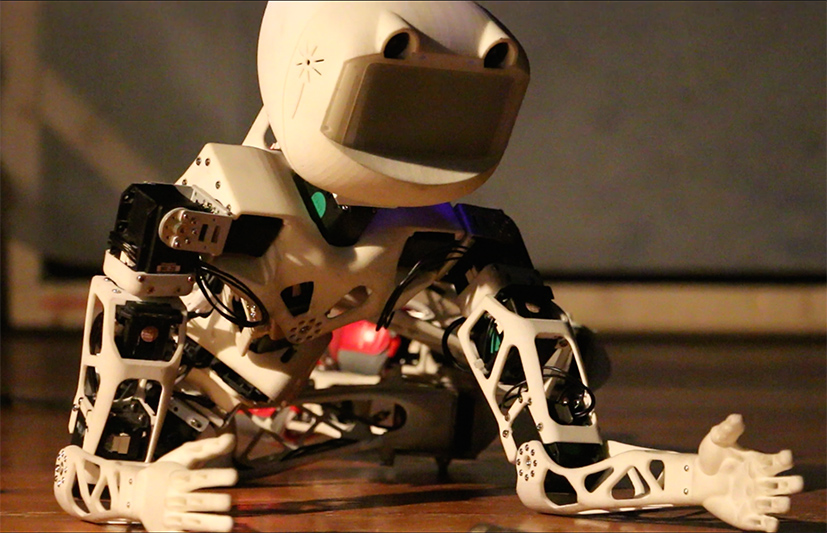
\includegraphics[width=0.46\linewidth]{ENP_img2.png}}
    \hfil
    \subfloat[][]{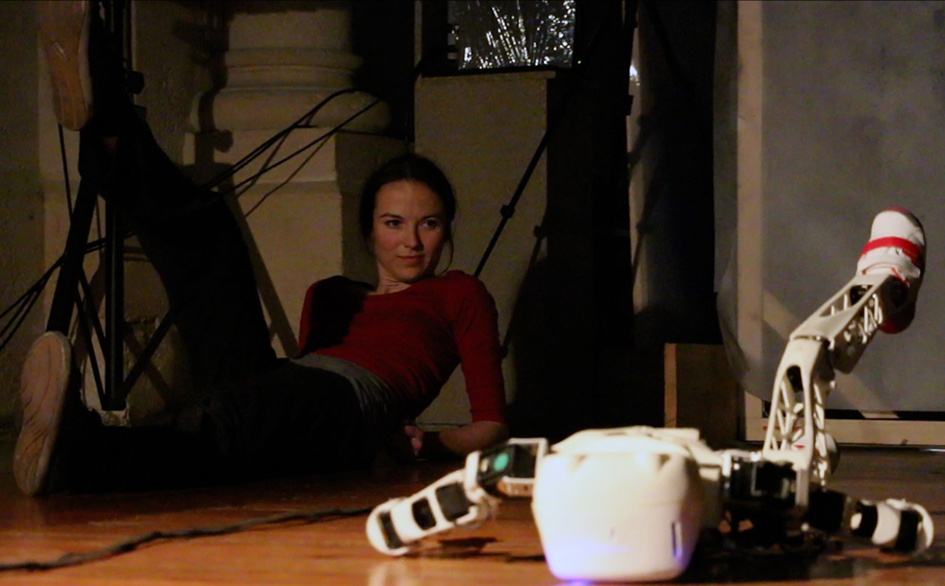
\includegraphics[width=0.46\linewidth]{art_floor.jpg}}\\
    \subfloat[][]{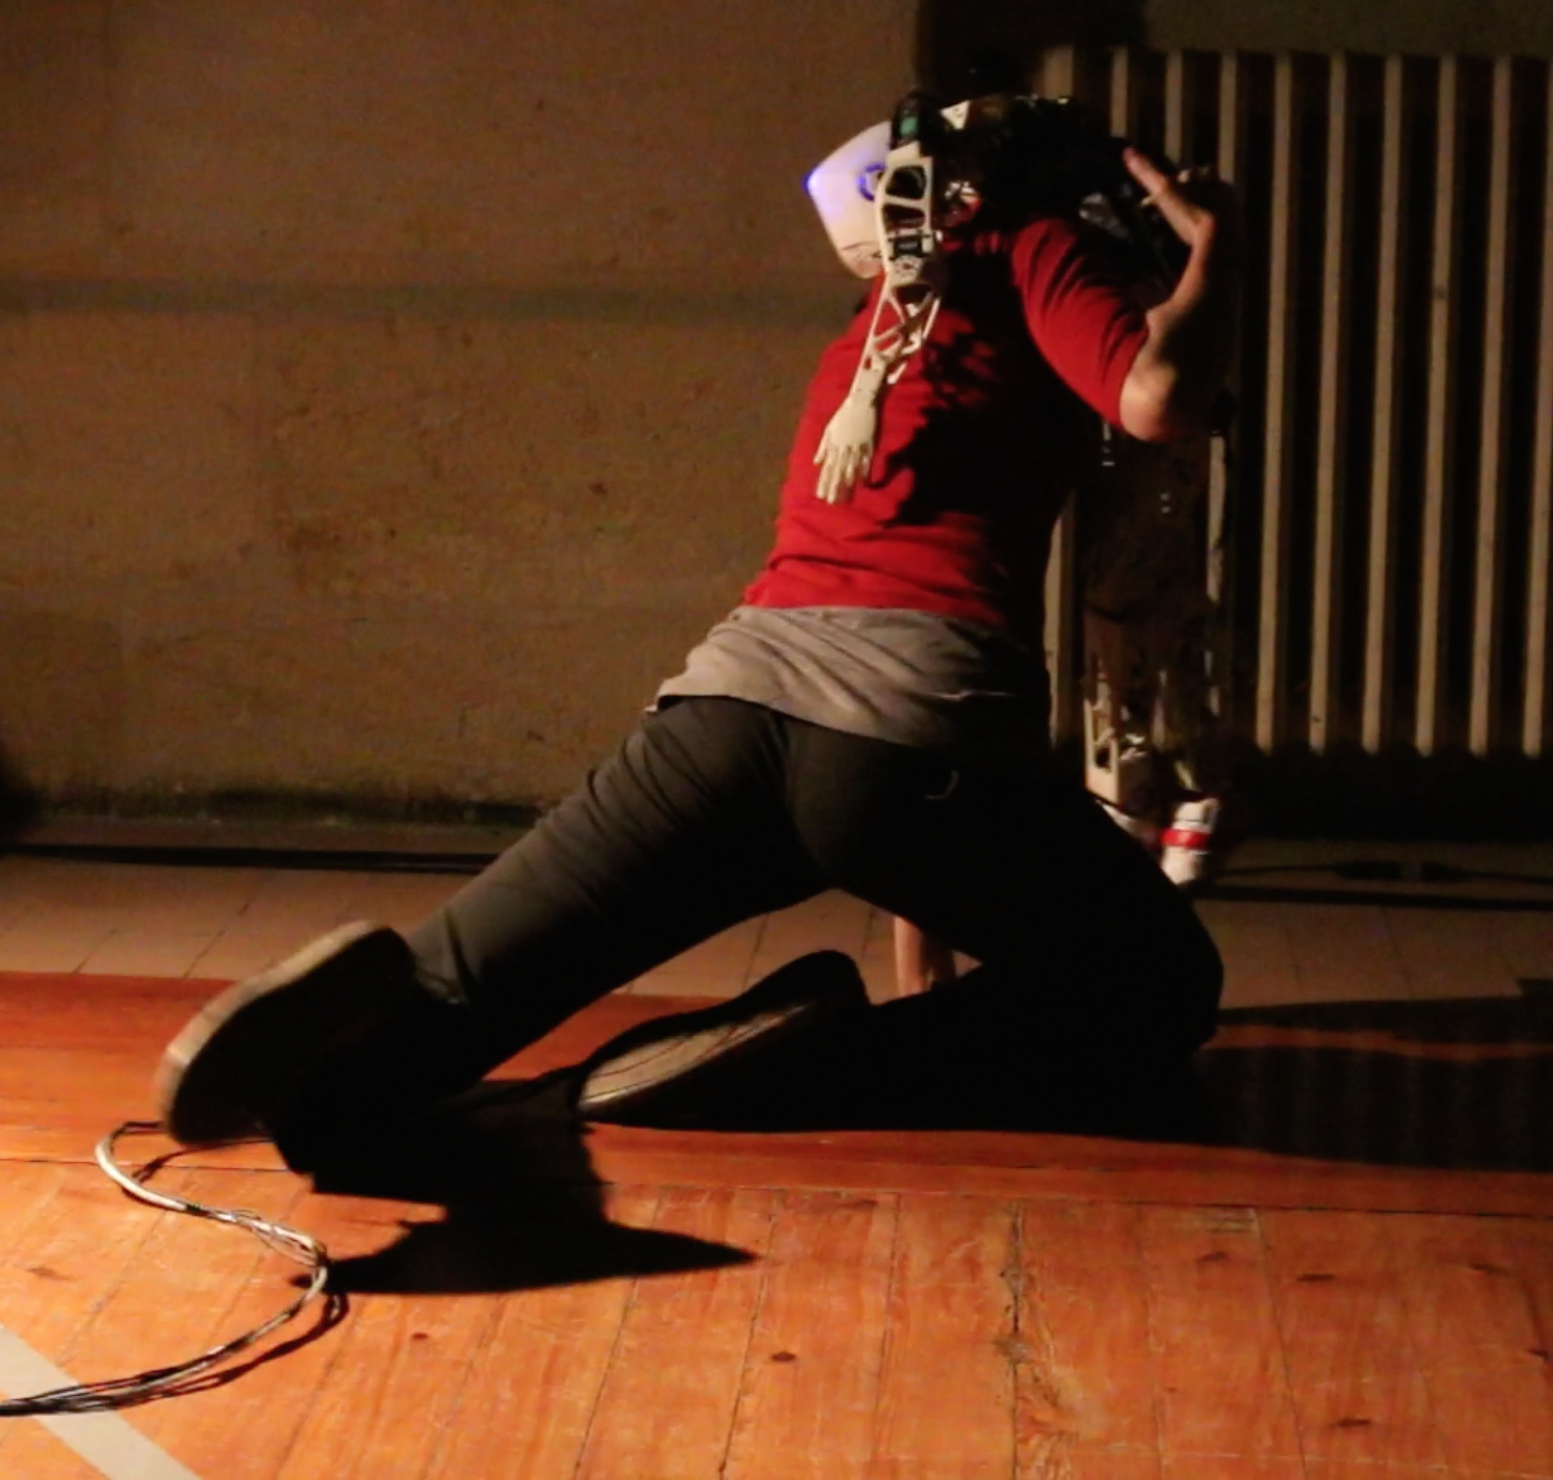
\includegraphics[height=5.3cm]{img6.png}}
    \hfil
    \subfloat[][]{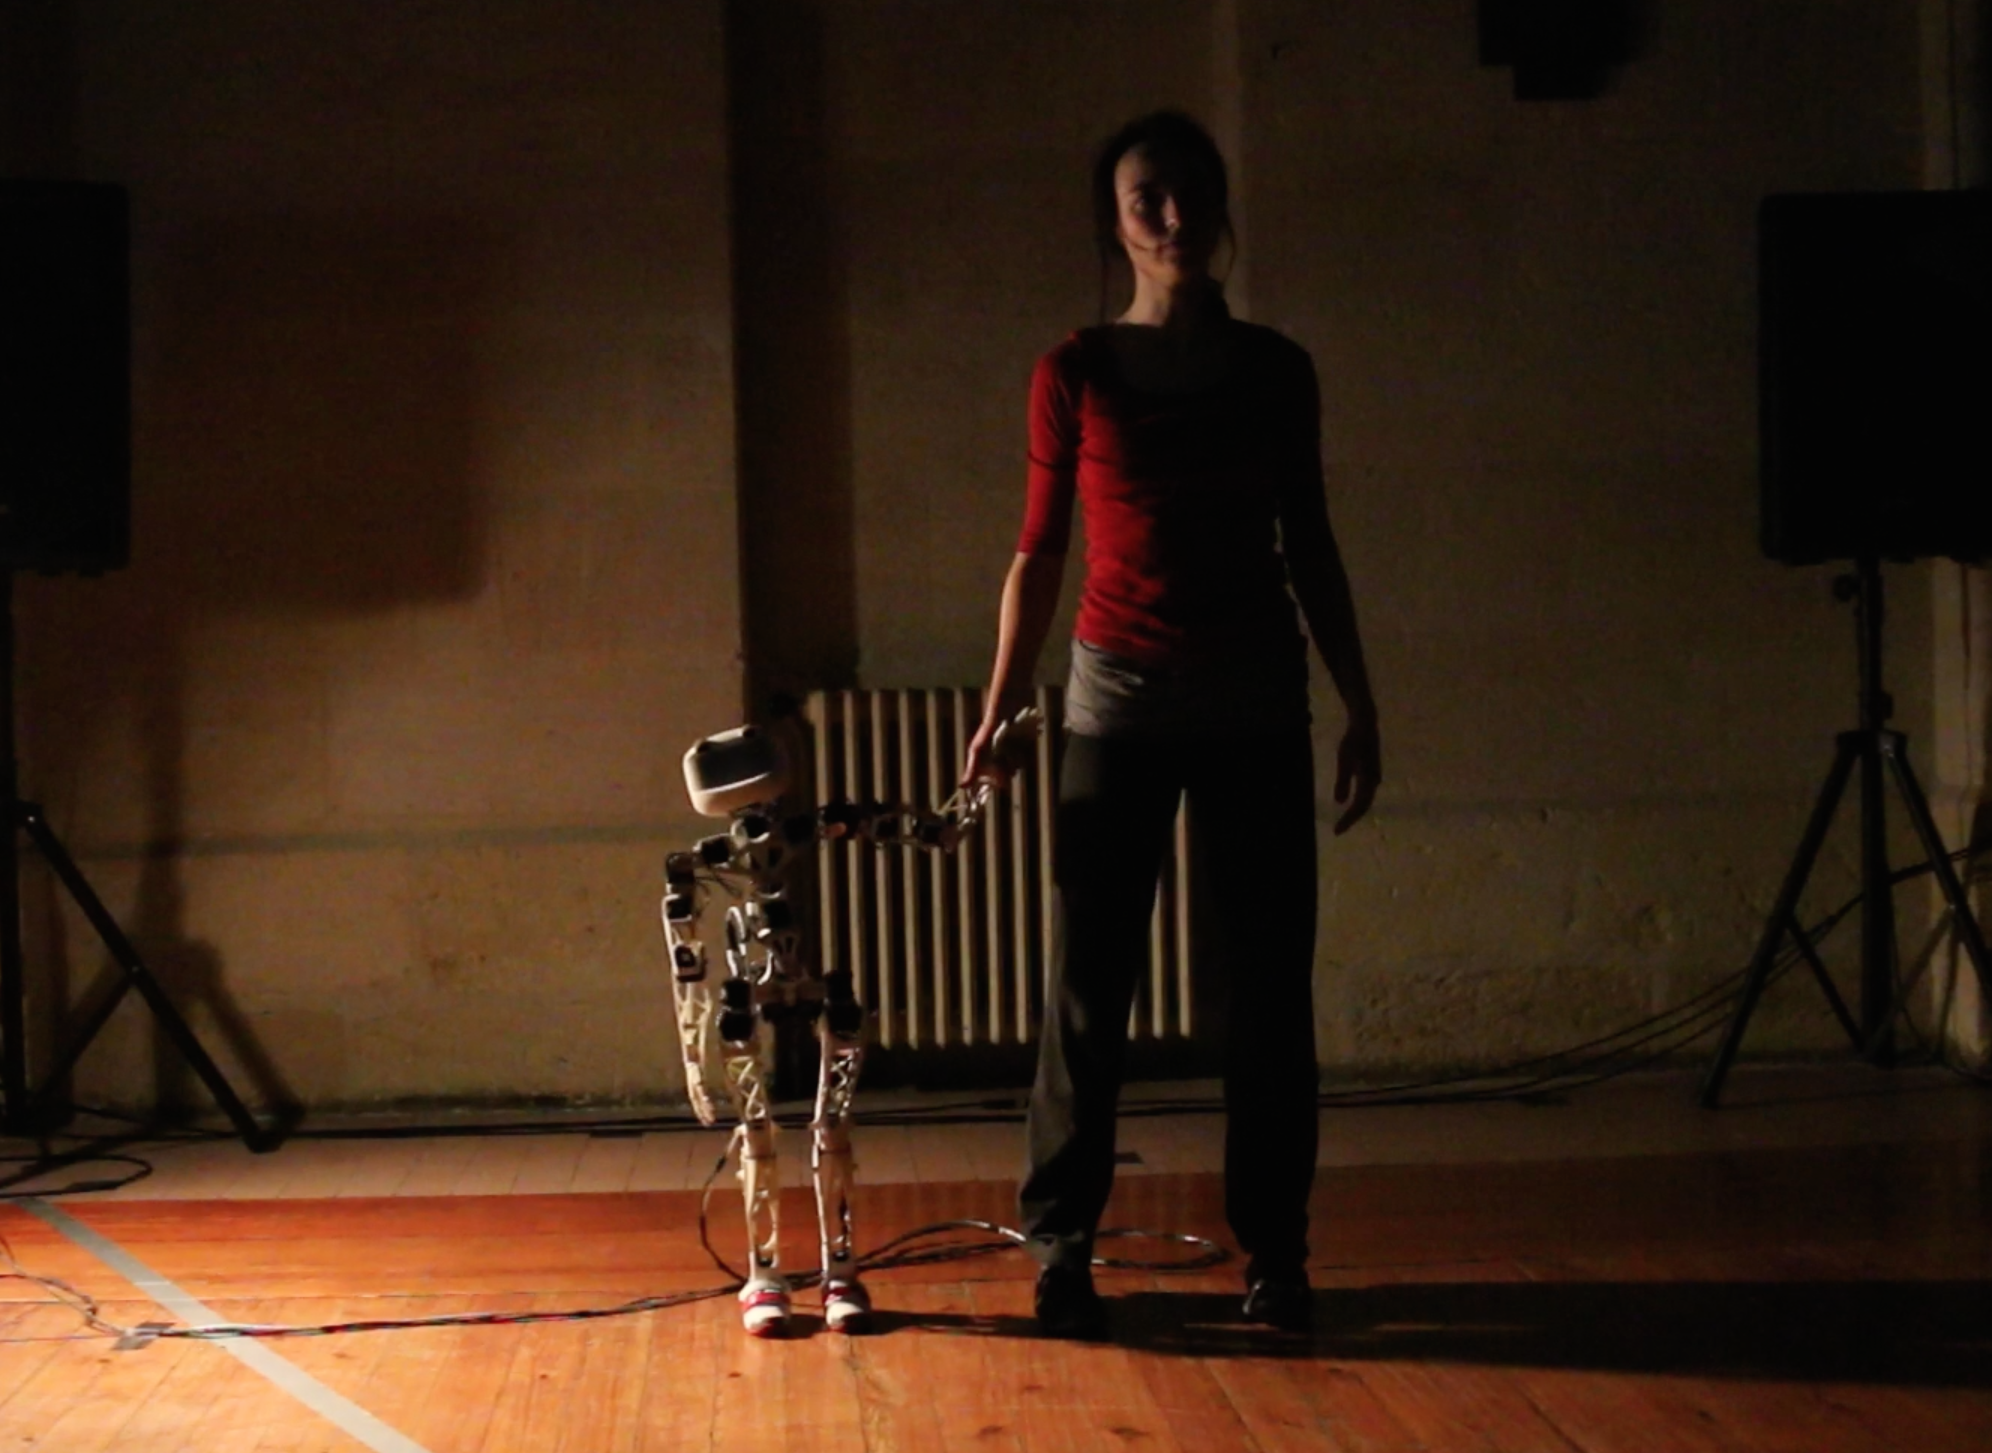
\includegraphics[height=5.3cm]{poppy_dancer_stand_up.png}}\\
    \subfloat[][]{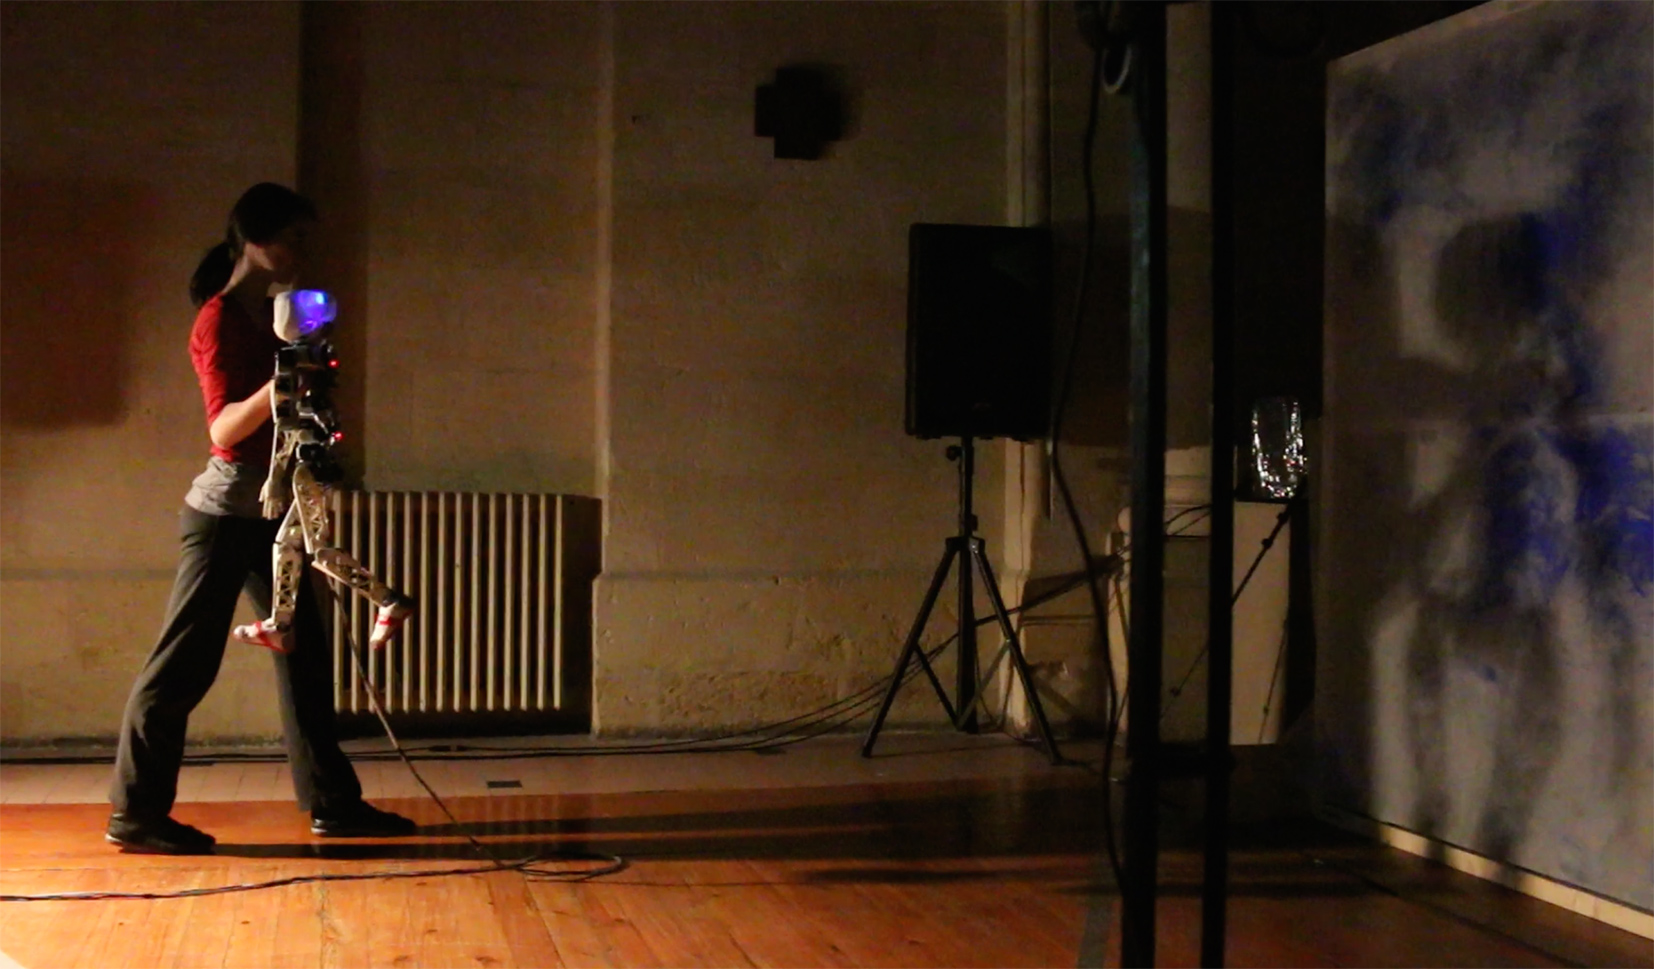
\includegraphics[width=0.95\linewidth]{img3.png}}
    \caption{}
    \label{fig:poppy_dance_performance}
\end{figure}


\subsection{Feedback} % (fold)

Unfortunately or fortunately, the use of Poppy by artists  in these workshops  was not without problems.(\figurename~\ref{fig:broken_poppy_residency}).

Firstly, it appears to be difficult for non-expert users to evaluate the real resistance of Poppy. After initially acting overly cautiously with it, they become overconfident about its robustness and no longer pay attention to signs indicating that the robot will break. The experiment with the little boy adding clay was quite destructive. Poppy spent almost 2 hours wrapped in cellophane withstanding kilos of clay, eventually it overheated and two motors in the hip and abs melted.
Thus adding a security system that alerts users when the robot is in a dangerous state appears to be a real necessity.  Otherwise non-expert users will regularly break motors without understanding why.

\begin{figure}[]
\centering
    \subfloat[][]{\includegraphics[height=4.5cm]{IMG_0019.jpg}}
    \hfil
    \subfloat[][]{\includegraphics[height=4.5cm]{IMG_0046.jpg}}
    \caption{}
    \label{fig:broken_poppy_residency}
\end{figure}

Secondly, the close interaction between Poppy and the dancer showed it is really complicated, when the robot is compliant, to avoid motors reaching dead-band. In addition, wires tend to tangle around motors and eventually unplug some of them. To avoid this recurrent problem, we built a primitive system on pypot  to check the state of each motor and stop it when it reached a given amplitude. Also, we are working on mechanical ways of avoiding the full-rotation of certain Poppy links.

Thirdly, the wires are really problematic; they caused a lot of problems throughout the residency. In the context of intensive use of the robot performing large amplitude motion, wires were solicited and eventually some of them became damaged, which provoked short-circuit and so destroyed some motors and micro-controllers.

During the residency, the ease of programming through the Pypot library permitted to design a simple interface allowing the dancer to physically sculpt novel movements, the softness of which could be dynamically controlled.

Pypot programing by demonstration is really basic: positions are recorded at 50hz and played. It is not at all optimized and even a bit bothersome to use because you cannot edit your moves. But this way of "programming" the robot has also a great advantage. The artist really appreciated sculptinggestures in this way rather than editing curves on a nice interface because she could really feel the weight of the robot and work on how to move its mass from one support to another. Finally, because Poppy is not over-actuated, it constrains motion to whom requiring the less power actuation and therefore leads to the creation of more natural motion.


\section{Discussion} % (fold)

The work the artists did was really amazing and they found unexpected potential in Poppy. Among them, the choreography Marie Aline Villard did was very elegant and sensitive. These movements put Poppy in the domain of sensitivity, rarely seen in humanoid robotics. This choreography is now often used for demonstration of the Poppy platform and closes the communication video showing Poppy being assembled in time-lapse \url{https://vimeo.com/96262428}.
Also, from a community impact point of view, the topic\footnote{\url{https://forum.poppy-project.org/t/artist-residency-etres-et-numerique/}} related to this experiment is by far the most followed subject of our forum.

But this work also showed the limits of Poppy. As for the Ergo-robots experience\footnote{Ergo-robots had to be functional for 5 months 8 hours per day. Our technologies have really participated in long-term experiments in the real world. In particular, the feedback we got from this experience greatly contributed to the methodology we built for the design of Poppy.}, the artist residency we did with  Poppy was really instructive. Firstly, Poppy has been used in totally unknown and unexpected/able situations, playing in pigments, dancing for 2 hours and so on were not on the development to-do list.
It was a real crash test for a novel experimental platform. Again, like in the ergo-robot experience, we learned the hard way how problematic the wires are. Most of the problems we had were due to damaged wires, which provoked short-circuit and eventually destroyed some motors and micro-controllers. It is a real problem in robotics right now, and it is really complicated to find a way to avoid it while keeping a modular and highly hackable robot.

We took note of each hardware problem to be solved for the release of the 1.0 version of Poppy and they are in progress. However, it would maybe not be enough (at the beginning) because it appears we also need to add specific software to monitor and protect the robot motors against overheating and overload. These protections are often task-dependent and the way we should handle it remains unclear. Therefore, the development will be done with the community in an iterative way until an efficient and robust solution is found.

Another problem for diffusion in the artistic community is the cost of the robot. Obtaining the \texteuro7000-8000 required to build a Poppy is really difficult and Artists are already having difficulty being paid so they have scarce funding for material.

An alternative could be to rely on the growing Fablab community~\parencite{anderson2012makers}. The collaboration between an artist and a Fablabs could at the same time, ensure technical support and assistance for using Poppy, avoid the funding problem by using Fablab's Poppy and promote local collaboration between complementary actors.

The interaction with Fablab is a very important point for the Poppy project, we will discuss it in the next chapter.

